\documentclass[aspectratio=169,10pt]{beamer}

\usetheme{default}
\setbeamertemplate{navigation symbols}{}
\setbeamersize{text margin left=0.55cm,text margin right=0.55cm}

\usepackage[T1]{fontenc}
\usepackage{lmodern}
\usepackage{booktabs}
\usepackage{graphicx}
\usepackage{array}
\usepackage{xcolor}
\usepackage{tikz}
\usetikzlibrary{arrows.meta}

\definecolor{nvblue}{HTML}{173B57}
\definecolor{nvteal}{HTML}{008C8C}
\definecolor{nvgray}{HTML}{42505A}
\definecolor{nvlight}{HTML}{F3F6F7}

\setbeamercolor{frametitle}{fg=nvblue}
\setbeamercolor{normal text}{fg=black,bg=white}
\setbeamercolor{block title}{fg=white,bg=nvblue}
\setbeamercolor{block body}{fg=black,bg=nvlight}
\setbeamerfont{frametitle}{series=\bfseries,size=\Large}
\setbeamerfont{block title}{series=\bfseries,size=\small}
\setbeamerfont{block body}{size=\scriptsize}
\setbeamertemplate{footline}{%
  \hfill{\tiny Lock-in update \insertframenumber/\inserttotalframenumber}\hspace{0.6em}\vspace{0.35em}
}

\newcommand{\code}[1]{\texttt{\scriptsize #1}}
\newcommand{\assetdir}{assets/lockin_progress}

\title{Lock-in Update}
\subtitle{Multipoint parked-frequency lock-in working end-to-end}
\date{May 7, 2026}

\begin{document}

\begin{frame}{Where the lock-in is now}
\vspace{-0.2em}
\begin{columns}[T,totalwidth=\textwidth]
\begin{column}{0.62\textwidth}
\begin{block}{What's working}
\begin{itemize}\setlength{\itemsep}{0.3em}
  \item Full pipeline runs end-to-end: ODMR sweep $\to$ parked-frequency plan $\to$ multipoint acquire $\to$ $\Delta f$ inference $\to$ B-vector reconstruction.
  \item All 16 parked frequencies measured in a single FPGA program (\code{MultipointLockinODMR}) — no more per-frequency upload overhead.
  \item Reference shot is now genuinely MW-off: a long ($\sim$1700 $\mu$s) relax delay between signal and reference lets the spins repolarize, so the reference no longer carries dip structure.
  \item Live mode builds the program once outside the batch loop and uses \code{pre\_init=False} — the per-batch peaking spike from 01\_basic is gone.
\end{itemize}
\end{block}
\end{column}
\begin{column}{0.34\textwidth}
\begin{block}{May 7 run snapshot}
\resizebox{\linewidth}{!}{%
\begin{tabular}{@{}ll@{}}
\toprule
ODMR source & \code{20260507\_140754} \\
Parked points & 16 \\
Transitions & 8 \\
Bias field & $-2.30,-2.99,-3.14$ mT \\
Single-batch acquire & 116 ms \\
Live run & 281 samples, 21.0 s \\
Live rate & 13.4 Hz \\
Vector rank-ok & 281 / 281 \\
\bottomrule
\end{tabular}
}
\end{block}
\end{column}
\end{columns}
\end{frame}

\begin{frame}{Reference shots are actually MW-off now}
\vspace{-0.4em}
\begin{columns}[T,totalwidth=\textwidth]
\begin{column}{0.56\textwidth}
\centering

\includegraphics[height=0.80\textheight,width=\linewidth,keepaspectratio]{\assetdir/odmr_signal_reference_contrast.png}
\end{column}
\begin{column}{0.40\textwidth}
\begin{block}{What changed}
\begin{itemize}\setlength{\itemsep}{0.35em}
  \item Each sweep point now grabs MW-on signal and MW-off reference in one pass.
  \item Long ($\sim$1700 $\mu$s) delay between the two integrations lets the always-on laser repolarize the spins, so the reference doesn't carry residual dip structure.
  \item The contrast trace = signal $-$ reference is what feeds parked-frequency planning.
\end{itemize}
\end{block}
\end{column}
\end{columns}
\end{frame}

\begin{frame}{Parked-frequency plan from the ODMR fit}
\vspace{-0.3em}
\begin{columns}[T,totalwidth=\textwidth]
\begin{column}{0.62\textwidth}

\includegraphics[width=\linewidth]{\assetdir/parked_frequency_overlay.png}
\end{column}
\begin{column}{0.36\textwidth}
\begin{block}{Plan output}
\centering
\tiny
\begin{tabular}{@{}rrrrr@{}}
\toprule
Blk & Center & Line & $f_-$ & $f_+$ \\
 & MHz & MHz & MHz & MHz \\
\midrule
1 & 2630.0 & 4.0 & 2629.0 & 2632.0 \\
2 & 2767.4 & 9.9 & 2764.0 & 2770.0 \\
3 & 2806.0 & 4.0 & 2803.0 & 2809.0 \\
4 & 2840.0 & 4.0 & 2837.0 & 2843.0 \\
5 & 2880.6 & 3.4 & 2878.0 & 2882.0 \\
6 & 2880.6 & 3.6 & 2878.0 & 2882.0 \\
7 & 2941.5 & 4.5 & 2939.0 & 2944.0 \\
8 & 2974.9 & 10.5 & 2971.0 & 2978.0 \\
\bottomrule
\end{tabular}
\end{block}
\begin{block}{Custom program}
\scriptsize
The 16 points aren't evenly spaced — they're the steepest-slope flank points of the 8 NV transitions. A stock QICK linear sweep can't hit non-uniform frequencies, hence \code{MultipointLockinODMR} on the next slide.
\end{block}
\end{column}
\end{columns}
\end{frame}

\begin{frame}{One FPGA program for all 16 parked points}
\vspace{-0.25em}
\begin{columns}[T,totalwidth=\textwidth]
\begin{column}{0.48\textwidth}
\begin{block}{What it does}
\begin{itemize}\setlength{\itemsep}{0.35em}
  \item One \code{MultipointLockinODMR} program holds the ASM for all 16 frequencies — uses \code{mw\_frequency\_register.set\_to(f)} inside \code{body()} to hop between them.
  \item Predicted FPGA work: 68 ms per batch (6.8 ms/rep $\times$ 10 reps). Measured first batch: 116 ms.
  \item Output: \code{multipoint\_lockin\_collected.csv} — one wide row per batch with \code{peak\_NN}, \code{peak\_NN\_ref}, \code{peak\_NN\_freq\_mhz}.
\end{itemize}
\end{block}
\begin{block}{Build once, not per batch}
\scriptsize
If you instantiate \code{MultipointLockinODMR} inside the batch loop, it re-uploads the FPGA program every iteration ($\sim$300 ms each — kills the speedup). Build once outside, then call \code{prog.acquire(progress=False)} in the loop.
\end{block}
\end{column}
\begin{column}{0.49\textwidth}
\begin{block}{Example columns from the wide CSV}
\centering
\tiny
\begin{tabular}{@{}rrrr@{}}
\toprule
Peak & Freq MHz & Signal ADC & Ref ADC \\
\midrule
01 & 2629.0 & 6529.6 & 6535.3 \\
02 & 2632.0 & 6539.4 & 6543.4 \\
09 & 2878.0 & 6502.5 & 6507.1 \\
10 & 2882.0 & 6488.6 & 6498.9 \\
15 & 2971.0 & 6499.1 & 6509.3 \\
16 & 2978.0 & 6499.2 & 6510.1 \\
\bottomrule
\end{tabular}
\end{block}
\begin{block}{Speedup vs the old loop}
\scriptsize
Old 17-program loop at \code{reps=100}: $\sim$6.6 s per batch, worse with network jitter. New multipoint at the same reps: $\sim$700 ms per batch after the one-time upload — about 10$\times$ faster.
\end{block}
\end{column}
\end{columns}
\end{frame}

\begin{frame}{Two-Point $\Delta f$ Formula}
\vspace{-0.4em}
\begin{columns}[T,totalwidth=\textwidth]
\begin{column}{0.58\textwidth}
\begin{block}{Derivation}
\small
Linearize the spectrum at each parked point as $f_0 \!\to\! f_0+\Delta f$:
\[
S_-(t)\approx b_- - m_-\,\Delta f,\quad
S_+(t)\approx b_+ - m_+\,\Delta f .
\]
Subtract to cancel common-mode drift:
\[
\Delta d_{\rm now}-\Delta d_{\rm ref}=(m_- - m_+)\,\Delta f .
\]
\[
\boxed{\;\Delta f_k=\dfrac{\Delta d_{\rm now}-\Delta d_{\rm ref}}{m_- - m_+},
\qquad
f_{{\rm new},k}=f_{0,k}+\Delta f_k\;}
\]
\end{block}
\end{column}
\begin{column}{0.40\textwidth}
\begin{block}{Symbols}
\scriptsize
$b_\pm,\ m_\pm$: PL and slope at $f_\pm$ from the reference ODMR.\\[0.15em]
$\Delta d_{\rm now}=S_+(t)-S_-(t)$;\ \ $\Delta d_{\rm ref}=b_+-b_-$.\\[0.15em]
$\Delta B_{{\rm proj},k}=\Delta f_k/\|\mathrm{d}f/\mathrm{d}B\|_k$.
\end{block}
\begin{block}{Block 4, latest batch}
\centering\tiny
\begin{tabular}{@{}lr@{}}
\toprule
$m_-$,\ $m_+$ & $-4.17{\times}10^{-4}$,\ $+5.36{\times}10^{-4}$\,/MHz \\
$\Delta d_{\rm now}-\Delta d_{\rm ref}$ & $-9.43{\times}10^{-4}$ \\
$\Delta f$ & $+0.990$ MHz \\
$f_{\rm new}$ & $2862.979$ MHz \\
\bottomrule
\end{tabular}
\end{block}
\end{column}
\end{columns}
\end{frame}

\begin{frame}{Why Denominator is $m_- - m_+$, Not $m_+ - m_-$}
\vspace{-0.6em}
\begin{columns}[T,totalwidth=\textwidth]
\begin{column}{0.50\textwidth}
\centering
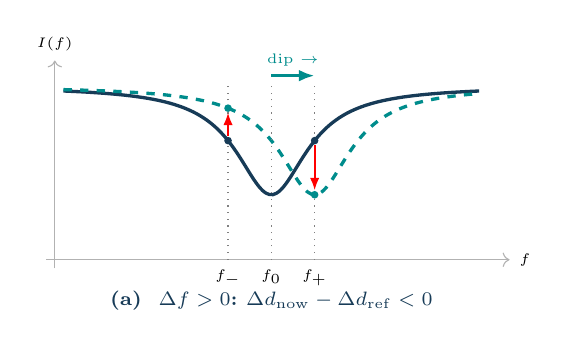
\begin{tikzpicture}[scale=0.55,every node/.style={font=\tiny}]
  \draw[->,gray!60] (-0.2,0) -- (10.5,0) node[right,black] {$f$};
  \draw[->,gray!60] (0,-0.2) -- (0,4.6) node[above,black] {$I(f)$};
  \draw[very thick,nvblue,smooth] plot[domain=0.2:9.8,samples=120]
    (\x,{4 - 2.5/(1 + ((\x-5)/1.0)^2)});
  \draw[very thick,dashed,nvteal,smooth] plot[domain=0.2:9.8,samples=120]
    (\x,{4 - 2.5/(1 + ((\x-6)/1.0)^2)});
  \draw[dotted,gray] (4,0) -- (4,4);
  \draw[dotted,gray] (5,0) -- (5,4);
  \draw[dotted,gray] (6,0) -- (6,4);
  \fill[nvblue] (4,2.75) circle (2.5pt);
  \fill[nvblue] (6,2.75) circle (2.5pt);
  \fill[nvteal] (4,3.5) circle (2.5pt);
  \fill[nvteal] (6,1.5) circle (2.5pt);
  \draw[-{Latex[length=1.6mm]},red,thick] (4,2.85) -- (4,3.4);
  \draw[-{Latex[length=1.6mm]},red,thick] (6,2.65) -- (6,1.6);
  \draw[-{Latex[length=2mm]},nvteal,very thick] (5,4.25) -- (6,4.25);
  \node[nvteal,above,font=\tiny] at (5.5,4.25) {dip $\to$};
  \node[below] at (4,0) {$f_-$};
  \node[below] at (5,0) {$f_0$};
  \node[below] at (6,0) {$f_+$};
  \node[nvblue,font=\scriptsize\bfseries] at (5,-0.95)
    {(a)\ \ $\Delta f>0$:\ $\Delta d_{\rm now}-\Delta d_{\rm ref}<0$};
\end{tikzpicture}
\end{column}
\begin{column}{0.50\textwidth}
\centering
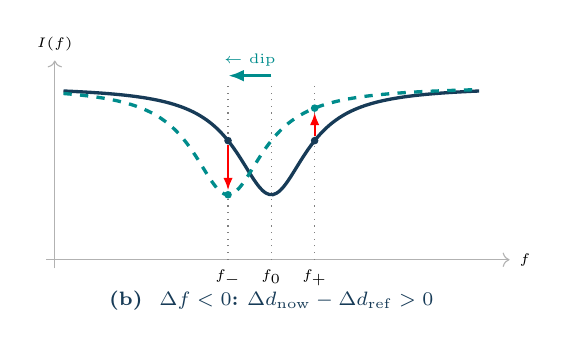
\begin{tikzpicture}[scale=0.55,every node/.style={font=\tiny}]
  \draw[->,gray!60] (-0.2,0) -- (10.5,0) node[right,black] {$f$};
  \draw[->,gray!60] (0,-0.2) -- (0,4.6) node[above,black] {$I(f)$};
  \draw[very thick,nvblue,smooth] plot[domain=0.2:9.8,samples=120]
    (\x,{4 - 2.5/(1 + ((\x-5)/1.0)^2)});
  \draw[very thick,dashed,nvteal,smooth] plot[domain=0.2:9.8,samples=120]
    (\x,{4 - 2.5/(1 + ((\x-4)/1.0)^2)});
  \draw[dotted,gray] (4,0) -- (4,4);
  \draw[dotted,gray] (5,0) -- (5,4);
  \draw[dotted,gray] (6,0) -- (6,4);
  \fill[nvblue] (4,2.75) circle (2.5pt);
  \fill[nvblue] (6,2.75) circle (2.5pt);
  \fill[nvteal] (4,1.5) circle (2.5pt);
  \fill[nvteal] (6,3.5) circle (2.5pt);
  \draw[-{Latex[length=1.6mm]},red,thick] (4,2.65) -- (4,1.6);
  \draw[-{Latex[length=1.6mm]},red,thick] (6,2.85) -- (6,3.4);
  \draw[-{Latex[length=2mm]},nvteal,very thick] (5,4.25) -- (4,4.25);
  \node[nvteal,above,font=\tiny] at (4.5,4.25) {$\leftarrow$ dip};
  \node[below] at (4,0) {$f_-$};
  \node[below] at (5,0) {$f_0$};
  \node[below] at (6,0) {$f_+$};
  \node[nvblue,font=\scriptsize\bfseries] at (5,-0.95)
    {(b)\ \ $\Delta f<0$:\ $\Delta d_{\rm now}-\Delta d_{\rm ref}>0$};
\end{tikzpicture}
\end{column}
\end{columns}
\vspace{0.5em}
\begin{block}{Sign self-consistency}
\scriptsize
Slope signs are fixed by the dip shape: $m_-<0$ (left flank descends),
$m_+>0$ (right flank ascends), so $m_- - m_+ < 0$ \emph{always}. The
numerator flips sign with the dip's direction (panels a, b above).
Combining: $(-)/(-) = +$ in (a) and $(+)/(-) = -$ in (b), so $\Delta f$
inherits the dip's true sign of motion. Flipping the denominator order
to $m_+ - m_-$ (always $>0$) would invert every $\Delta f$.
\end{block}
\end{frame}


\begin{frame}{Live run: drift and noise floor}
\vspace{-0.35em}
\begin{columns}[T,totalwidth=\textwidth]
\begin{column}{0.58\textwidth}

\includegraphics[width=\linewidth]{\assetdir/live_delta_f_timeseries.png}
\end{column}
\begin{column}{0.40\textwidth}
\begin{block}{Run summary}
\begin{itemize}\setlength{\itemsep}{0.25em}
  \item Live CSV \code{20260507\_141355}.
  \item 281 batches over 21.0 s $\to$ 13.4 Hz update rate.
  \item Per-batch timing: predicted 68 ms; actual median 12 ms, p95 15 ms, max 17 ms.
  \item Watchdog never fired.
\end{itemize}
\end{block}
\begin{block}{Per-block stats}
\centering
\tiny
\begin{tabular}{@{}rrrr@{}}
\toprule
Blk & mean $\Delta f$ & std $\Delta f$ & std $\Delta B$ \\
 & MHz & MHz & uT \\
\midrule
1 & -0.211 & 0.354 & 12.6 \\
2 & -0.062 & 0.172 & 6.1 \\
3 & -0.583 & 0.460 & 16.3 \\
4 & +0.973 & 0.619 & 22.3 \\
5 & -0.645 & 0.102 & 7.4 \\
6 & -0.723 & 0.099 & 7.2 \\
7 & +0.024 & 0.279 & 9.9 \\
8 & -0.201 & 0.128 & 4.6 \\
\bottomrule
\end{tabular}
\end{block}
\end{column}
\end{columns}
\end{frame}

\begin{frame}{Inferred peak frequencies (live)}
\vspace{-0.55em}
\begin{columns}[T,totalwidth=\textwidth]
\begin{column}{0.49\textwidth}

\includegraphics[width=\linewidth]{\assetdir/live_new_peak_frequency_top.png}
\end{column}
\begin{column}{0.49\textwidth}

\includegraphics[width=\linewidth]{\assetdir/live_new_peak_frequency_bottom.png}
\end{column}
\end{columns}
\vspace{0.25em}
{\tiny Each block: $f_{\rm new}(t)=f_0+\Delta f(t)$ in solid, with the dashed reference $f_0$ from the ODMR calibration.}
\end{frame}

\begin{frame}{B-field reconstruction output}
\vspace{-0.35em}
\begin{columns}[T,totalwidth=\textwidth]
\begin{column}{0.58\textwidth}

\includegraphics[width=\linewidth]{\assetdir/live_bfield_components.png}
\vspace{0.2em}

\includegraphics[width=\linewidth]{\assetdir/live_bfield_magnitude.png}
\end{column}
\begin{column}{0.40\textwidth}
\begin{block}{Reconstruction stats}
\begin{itemize}\setlength{\itemsep}{0.3em}
  \item Input: wide live CSV from the 281-sample run above.
  \item Samples: 281; rank-ok: 281/281.
  \item Matrix condition number: 14.08.
\end{itemize}
\end{block}
\begin{block}{Vector component stats}
\centering
\tiny
\begin{tabular}{@{}rrrr@{}}
\toprule
Comp. & Mean uT & Std uT & Range uT \\
\midrule
$\Delta B_x$ & 18,923 & 81,622 & -351,633 to 248,403 \\
$\Delta B_y$ & -290,071 & 221,862 & -942,851 to 688,841 \\
$\Delta B_z$ & 79,653 & 104,794 & -323,599 to 634,124 \\
\bottomrule
\end{tabular}
\end{block}
\begin{block}{What's next}
\scriptsize
$\Delta B$ magnitudes are huge — likely the bias hasn't been subtracted yet, or the inversion needs a sanity check against a known applied field. Also want to replot \code{peak\_01} vs \code{acq\_seconds} from the CSV (outside the live cell) to confirm there's no batch-edge timing spike hiding in the data.
\end{block}
\end{column}
\end{columns}
\end{frame}

\end{document}
